\section{Time box 4}
\listoftodos
\subsection{Time box planning}
\begin{figure}[H]
	\begin{centering}
		\missingfigure{Updated timebox figure}
		%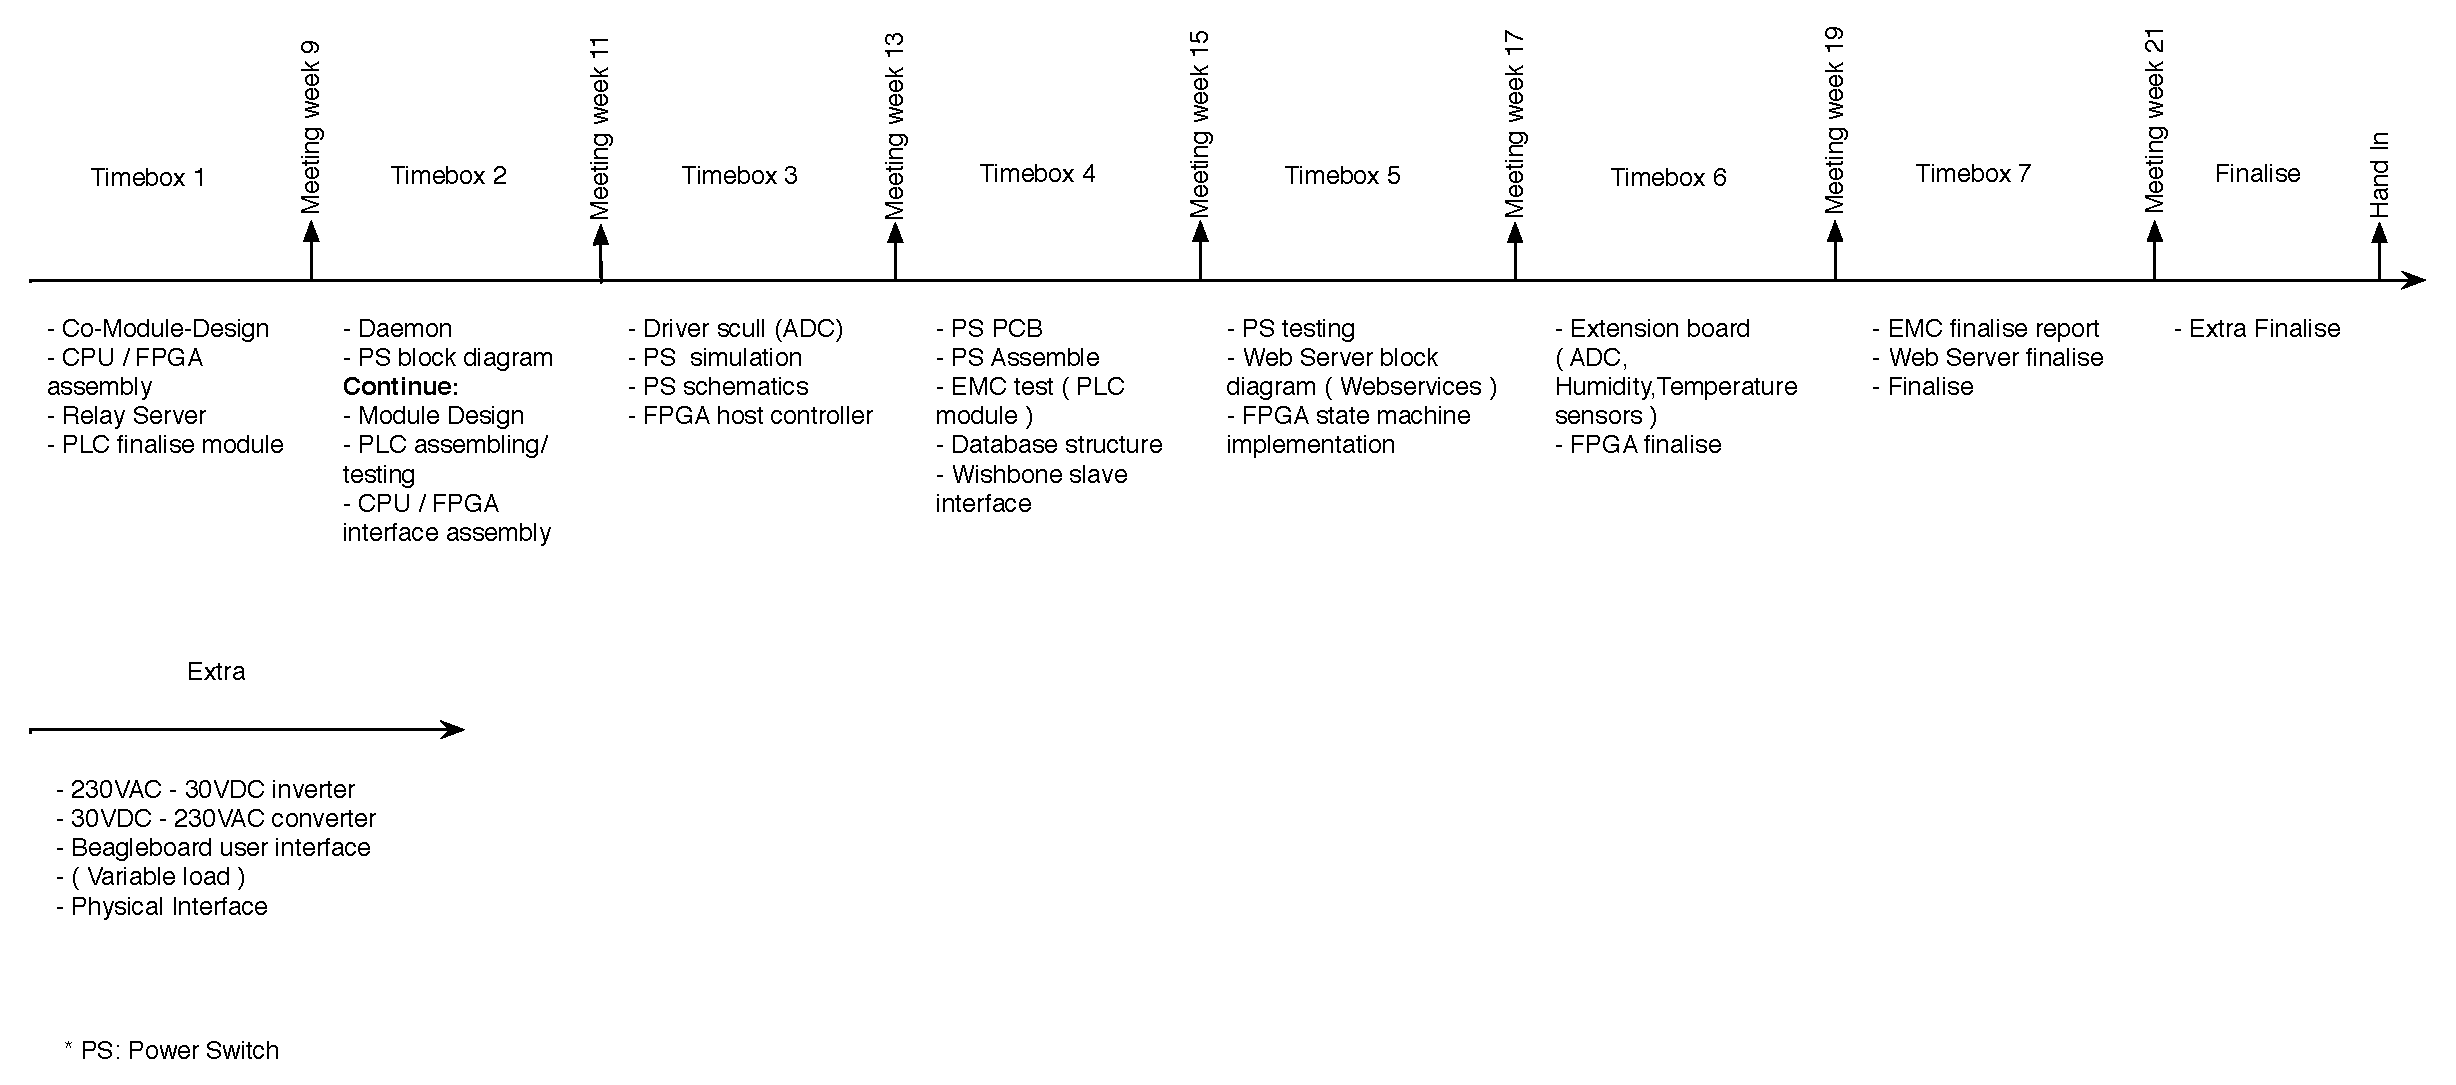
\includegraphics[width=1.0\textwidth]{images/tb_r3.pdf}
		%\caption{Updated time-box}
	\end{centering}
\end{figure}
\subsubsection{Work to be done in this time box}
\begin{itemize}
	\item Driver
	\begin{itemize}
		\item \todo[inline]{edit here Dennis}
	\end{itemize}
	\item Database
	\begin{itemize}
		\item \todo[inline]{edit what you like and bake a cake}
	\end{itemize}
	\item Physical interface
	\begin{itemize}
		\item Wishbone slave interface
		\item Switch driver
		\item LED driver
	\end{itemize}
\end{itemize}
\paragraph{Description:}
\begin{description}
	\item[Driver] \todo[inline]{edit here Dennis}
	\item[Database] \todo[inline]{edit here Jesus}
	\item[Physical interface] is the light indication and the switches that shall be on the physical hub interface
\end{description}
\subsubsection{Time planning}
\begin{table}[H]
\centering
	\begin{tabular}{|l|c|c|c|c|}
		\hline
		~			& Driver		& Database	& Physical interface\\ \hline
		Estimation	& xx			& 10		& 12				\\
		Actual		& xx			& xx		& 15				\\
		Developer	& Dennis		& Paulo		& Theis				\\
		\hline
	\end{tabular}
	\caption{Estimation and actual time used on the project}
\end{table}
\subsection{Driver - Dennis}
%			intro
%			
%					verification specification
%					deployment specification
%					
%			Analysis
%	
%	                Refactored block diagram
%	                Refactored class diagram
%	                Detailed use cases
%	                User interface specification
%	                System interface specification
%	                Dimensioning specification 
%	
%	        Design
%	
%	                UML/SysML deployment view(s)
%	                Mechanical specifications and dimensioning
%	                HW module specification per block
%	                UML SW deployment view
%	                Class specification
%	                Refactored class diagram
%	                Use case scenarios specifications
%	                Sequence diagrams 
%	
%	        Implementation
%	
%	                Mechanical drawings with details explained
%	                Electronic diagrams with details explained
%	                Source code with details explained
%	                Description of integration 
%	
%	        Verification
%	
%	                Module tests
%	                Integration tests
%	                Acceptance test
\subsection{Database - Paulo}
%		Intro

Each module in the system have sensors which send data to be stored and shown to the user. As such, data have to be stored in a convenient and consistent way. A MySQL database is used. All data stored have to be present in a web interface the integration between this type of data base and a server-side scripting ( PHP ) keeps the development faster and completely open source.
A database have to be consistent, flexible and efficient so no data is lost or repeated when a value is send to it.
%
%			Verification specification
\subsubsection{Verification specification}
A LAMP ( Linux Apache MySQL PHP ) web server is implemented at the development environment used to build the uClinux image. This use a linux distribution CENTOS virtual machine in which the web server was built ( how to build the web server explanation further in this documentation ).
For an easy and fast verification and development of the database a phpMyAdmin web application is installed at the server.
The verifications can be found at the end of this section.

%			Deployment specification
\subsubsection{Deployment specification}
\missingfigure{Have no idea what this should be}

%		Analysis
%	
%	                Refactored block diagram
%	                Refactored class diagram
%	                Detailed use cases
%	                User interface specification
%	                System interface specification
%	                Dimensioning specification 
\subsubsection{Analysis}
The analysis of the system information and requirements is fundamental to the development of a database. 
\paragraph{Requirements}
	\begin{itemize}
		\item Jan is looking at the web interface for the energy hub. From where he can see the status for each modules connected to it
in a graphically way.
		\item A new energy module is connected to the hub, Jan opens the web interface for the energy hub, he logs in the administrator section of the system
to start, stop or see a more detailed overview of each module.
		\item Jan arrives at the university in the morning and an email was send to him reporting a failure in the green energy system, he login to the administrator web interface, and he can see what the problem might be, and if it's possible to solve it directly on the interface.
	\end{itemize}

From this requirements given by the customer the relevant information for the database development is filtered:
	\begin{itemize}
		\item The status of each module have to be show.
		\item A detailed overview of each module such as current production (Voltage, Current, Power, etc.), efficiency of the module, etc.
		\item Errors have to be reported to the system administrator / maintainer.
	\end{itemize}
	
In a deeper analysis of the information system for the power energy hub, some technical data is needed to be stored such as:
	\begin{itemize}
		\item Each module have is unique id, this is similar to the MAC address, this way when a module is connected is possible to check if the module have been connected before, so the data can be stored for the same module instead of instantiate a new module which can generate ambiguous data.
		\item Three types of modules are defined: input, output and bidirectional. This are seen from the power hub point of view where inputs are producers ( solar panels, wind turbine, ... ), output are consumers ( Inverter, 30V output socket ) and bidirectional ( C.A.E.S, batteries, ...).
	\end{itemize}

%	        Design
%	
%	                UML/SysML deployment view(s)
%	                Mechanical specifications and dimensioning
%	                HW module specification per block
%	                UML SW deployment view
%	                Class specification
%	                Refactored class diagram
%	                Use case scenarios specifications
%	                Sequence diagrams 
%	
\subsubsection{Design}
The design of the database as part of its development is fundamental for a overview of the system, this is done with the use of data sets and data models. With data sets a detailed description of each table in the 

\lineparagraph{Data sets}
From the system information analysis a basic tabular structure is designed for a better understanding and low level overview of the database, this is called data set structure.
\\\\
TYPE(ID\_TYPE, TYPE);

\begin{table}[H]
\centering
	\begin{tabular}{| p{2cm} | p{10cm} |}
		\hline
		ID\_TYPE & Auto increment integer, a new id number is generated when a different type is needed to the system. \\\hline
		TYPE & Describe the type name for example: Input, output, bidirectional, etc.\\\hline
	\end{tabular}
\end{table}

STATUS(ID\_STATUS, STATUS);

\begin{table}[H]
\centering
	\begin{tabular}{| p{2cm} | p{10cm} |}
		\hline
		ID\_STATUS & Auto increment integer, a new id number is generated when a different status is needed to the system. \\\hline
		STATUS & Describe the status name for example: Running, stopped, warning, etc.\\\hline
	\end{tabular}
\end{table}


MODULES(ID\_MODULE, UNIQUE\_ID, ID\_TYPE, ID\_STATUS, NAME);

\begin{table}[H]
\centering
	\begin{tabular}{| p{2cm} | p{10cm} |}
		\hline
		ID\_MODULE & Auto increment integer, a new id number is generated every time an unknown module is connected. \\\hline
		UNIQUE\_ID & Module unique ID, this id as primary key ensures that no module with is repeated in the database.\\\hline
		ID\_TYPE & This is a foreigner key for the table type, this way if some other type of module is needed it can be dynamical add. \\\hline
		ID\_STATUS & This is a foreigner key for the table status, this way if some other status to the module is needed it can be dynamical add. \\\hline
		NAME & The name of the module for example, Solar Panel, wind turbine, battery. \\\hline
	\end{tabular}
\end{table}
As a requirement the database have to store the measurement  from different modules, the common and minimal measurements needed from the modules are current and voltage. So a log data set is created.
\\\\
LOGS(ID\_LOG, ID\_MODULE, DATE\_TIME, PORT, CURRENT, VOLTAGE);

\begin{table}[H]
\centering
	\begin{tabular}{| p{2cm} | p{10cm} |}
		\hline
		ID\_LOG & Auto increment integer, a new id number is generated every time a measurement is add. \\\hline
		ID\_MODULE & This is a foreigner key for the table modules, this allow the system to know from which module correspond the measurement .\\\hline
		DATE\_TIME & Date and time of the measurement is saved so it can be plotted or in case of a lower efficiency a detailed history can analysed. \\\hline
		PORT & Defines in which port or the energy hub the module is connected in the time of the measurement. \\\hline
		CURRENT & Current measurement. \\\hline
		VOLTAGE & Voltage measurement. \\\hline
	\end{tabular}
\end{table}

At this point the database can initialise a new module or identified if the module where connected before, change the status for each module and add new measurements for each module. ( Verification 1, 2 and 3 )

Measurements are add to the database every \todo{Time between measurements}, which in a non-stop system database size could be a problem, to avoid this situation a wrapper data set is created. This will store an average of values between a time span for each module, allowing the customer either to erase the values from the log or export them out from the database. Crucial data can be lost in this step for example the port history in case of troubleshooting, and precise date and time which would not allow the precise plot of data. 

WRAPPER(ID\_WRAP, ID\_MODULE, DATE\_FROM, DATE\_TO, AVG\_CURRENT, AVG\_VOLTAGE);

\begin{table}[H]
\centering
	\begin{tabular}{| l | p{10cm} |}
		\hline
		ID\_WRAP & Auto increment integer, a new id number is generated every time an wrap is needed. \\\hline
		ID\_MODULE & This is a foreigner key for the table modules, this allow the system to know from which module correspond the values .\\\hline
		DATE\_FROM & Date and time of the time span start. \\\hline
		DATE\_TO & Date and time of the time span end. \\\hline
		AVG\_CURRENT & Average current measurements. \\\hline
		AVG\_VOLTAGE & Average voltage measurements. \\\hline
	\end{tabular}
\end{table}

The system is now able to decrease the amount of space needed using a time span and average values. ( Verification 4 )

During the verification process some problems related to the flexibility of the database were found:
	\begin{itemize}
		\item Problem 1: The Photovoltaic and Wind Turbine modules have more measurements to be stored then only current and voltage, for example velocity and direction of the wind, sun position, etc.
		\item \todo{Meeting with martin anytime this week to talk about the database structure}
	\end{itemize}

\paragraph{Problem 1}
In the design of this database it was assumed that all the modules would only save to the database the current and voltage. But during the verification process, the designed database was not flexible enough by the type of measurements being restrict to only current and voltage.

	\begin{itemize}
		\item How to make the database more flexible so it would allow inserting different measurements for different modules?
	\end{itemize}

Different approaches were made:
	
	\begin{itemize}
		\item Option 1: Create a new table for each new module that have extra measurements and add the ID\_EXTRA to the logs table.
		\item Option 2: Give different unique ids to the sensors and relate them to their modules, so the log will store the sensor measurement.
	\end{itemize}

Option 1 is not consistent since when a new module is connected a new table have to be created for that module with the needed measurement units.\\
Option 2 is the most reliable and the implemented one. A table Units and Sensors were created:\\

SENSOR(ID\_SENSOR, ID\_MODULE, ID\_UNITS);

\begin{table}[H]
\centering
	\begin{tabular}{| p{2cm} | p{10cm} |}
		\hline
		ID\_SENSOR & Auto increment integer, a new id number is generated when a different sensor is needed to the system. \\\hline
		ID\_MODULE & This is a foreigner key for the table sensors, this allow the system to know from which module correspond the sensor, being a primary key with the id\_sensor, this way each sensor correspond to only one module .\\\hline
		ID\_UNITS & This is a foreigner key for the table units, this allow the system to know which units the sensor is measuring.\\\hline
	\end{tabular}
\end{table}

UNITS(ID\_UNIT, UNIT);

\begin{table}[H]
\centering
	\begin{tabular}{| p{2cm} | p{10cm} |}
		\hline
		ID\_UNIT & Auto increment integer, a new id number is generated when a different unit is needed to the system. \\\hline
		UNIT & Describe the unit name for example: A, V, deg ,m/s,etc. (Ampere, Volt, Degrees, Velocity)\\\hline
	\end{tabular}
\end{table}

In table wrapper and logs the ID\_MODULE was replaced with ID\_SENSOR. The database becomes more flexible since at anytime a module with new unknown sensors can be add and a sensor can be added to a existent module and the values will always be saved and retrieved to the user with the appropriat measurement units.

\lineparagraph{Data Model}
Data model is a high-level overview of the database structure. At this stage data sets are translated to a logic structure with the relationship between tables.

\begin{figure}[H]
	\begin{centering}
		%\missingfigure{Updated timebox figure}
		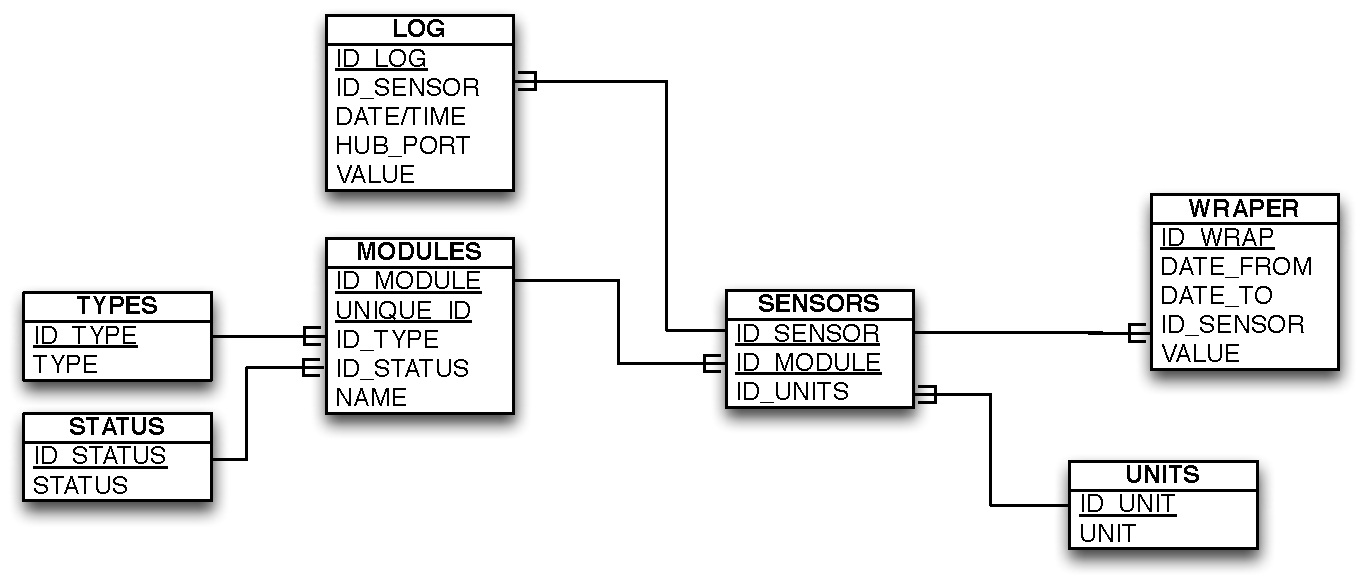
\includegraphics[width=1.0\textwidth]{images/db_structure.pdf}
		\caption{Data Model Structure}
	\end{centering}
\end{figure}


%	        Implementation
%	
%	                Mechanical drawings with details explained
%	                Electronic diagrams with details explained
%	                Source code with details explained
%	                Description of integration 
%	
\todo{White space after a code box is toooooo big.}
\subsubsection{Implementation}
Using the development environment virtual machine with the linux distribution CENTOS, a AMP ( Apache MySQL PHP ) web server is implemented, this way the web application phpMyAdmin is installed which simplifies the implementation of the database.

\lineparagraph{Webserver Implementation}
A LAMP ( Linux Apache MySQL PHP ) web server is implemented, this is explains step by step how to implement this kind of web server on a linux CENTOS OS.
\begin{itemize}
% Apache Install		
		\item Installing Apache and bring the server up.\\
			Install daemon that is going to handle HTTP requests on port 80. ( Apache )
			\begin{lstlisting}[language=c, stepnumber=0, tabsize=1]
				# yum install httpd
			\end{lstlisting}
			Start Apache in background.
			\begin{lstlisting}[language=c, stepnumber=0, tabsize=1]
				# /etc/init.d/httpd start
			\end{lstlisting}			
			Testing the web server. ( Verification 5 )
			\begin{figure}[H]
				\begin{centering}
					%\missingfigure{Webserver first page}
					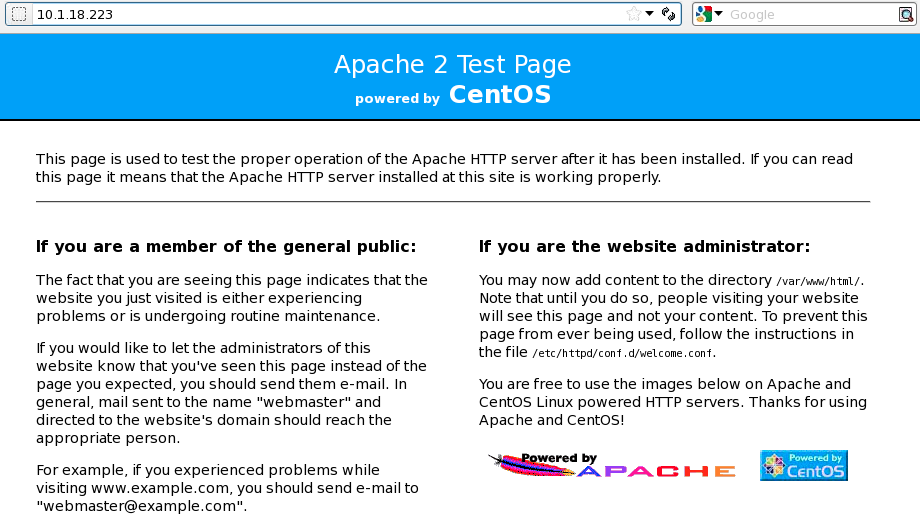
\includegraphics[width=1.0\textwidth]{images/first_web.png}
					\caption{First page apache server running}
				\end{centering}
			\end{figure}
% MySQL Install			
		\item Installing MySQL and bringing the server up\\
			Install MySQL server and client.
			\begin{lstlisting}[language=c, stepnumber=0, tabsize=1]
				# yum install mysql-server mysql
			\end{lstlisting}
			Start MySQL server in background.
			\begin{lstlisting}[language=c, stepnumber=0, tabsize=1]
				# /etc/init.d/mysqld start
			\end{lstlisting}
			Testing the MySQL server ( Verification 6 )
			\begin{lstlisting}[language=c, stepnumber=0, tabsize=1]
				# mysql
			\end{lstlisting}
			Server up and running when the follow response is given.
			\begin{lstlisting}[language=c, stepnumber=0, tabsize=1]
				Welcome to the MySQL monitor.  Commands end with ; or \g.
				Your MySQL connection id is 12
				Server version: 5.0.95 Source distribution

				Copyright (c) 2000, 2011, Oracle and/or its affiliates. All rights reserved.

				Oracle is a registered trademark of Oracle Corporation and/or its
				affiliates. Other names may be trademarks of their respective
				owners.

				Type 'help;' or '\h' for help. Type '\c' to clear the current input statement.

				mysql> 
			\end{lstlisting}
			At this moment the database is set with username root and an empty password. For security reasons a password is set for the MySQL server.\\\\
			Changing MySQL root password
			\begin{lstlisting}[language=c, stepnumber=0, tabsize=1]
				mysql> USE mysql;
				mysql> UPDATE user SET Password=PASSWORD('new password') WHERE user='root';
				mysql> FLUSH PRIVILEGES;
			\end{lstlisting}
			With the instruction 'USE mysql' the database directory mysql is open, 'UPDATE user SET Password=PASSWORD ('new password') WHERE user='root';' the password for the user 'root' is updated to the desired one. 'FLUSH PRIVILEGES' erases the privileges in cache and reloads the privileges in the MySQL server.
% PHP Install
		\item Installing PHP \\
		Install PHP scripting language and necessary modules for MySQL server.
		\begin{lstlisting}[language=c, stepnumber=0, tabsize=1]
			# yum install php php-mysql
		\end{lstlisting}
			php: scripting language compiler\\
			php-mysql: mysql functions to be called from a PHP script\\
		\\
		Testing PHP by creating a file in the web server documents root. /var/www/html/test.php. ( Verification 7 )
		\begin{lstlisting}[language=php, stepnumber=0, tabsize=1]
			//test.php
			<?php
				// Shows the in use PHP configuration file.
				phpinfo();
			?>
		\end{lstlisting}
		Accessing in the web browser to the web server ip address http://10.1.18.223/test.php
		\begin{figure}[H]
			\begin{centering}
				%\missingfigure{PHP info web page on the browser}
				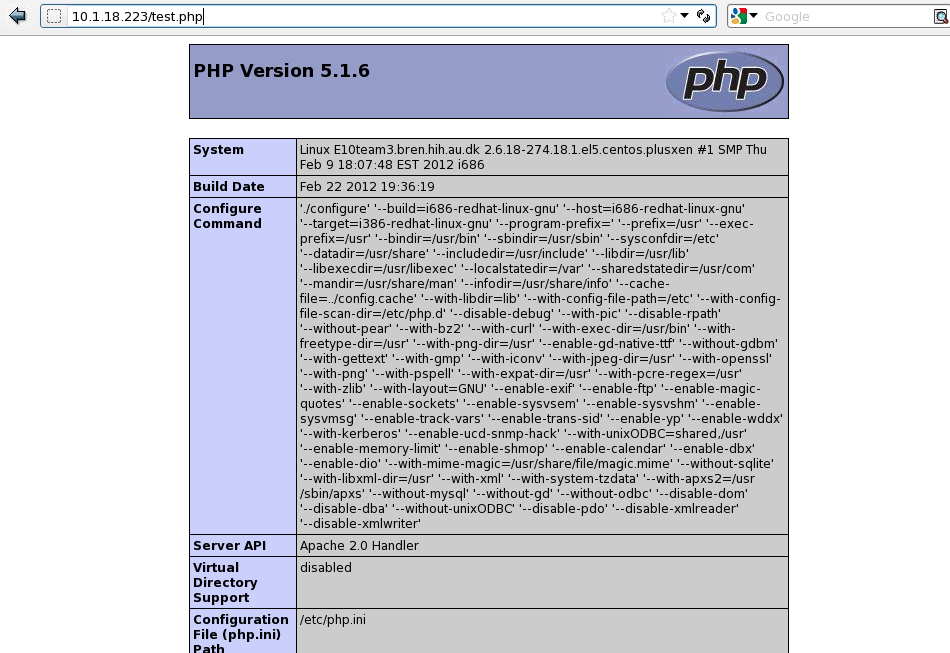
\includegraphics[width=1.0\textwidth]{images/php_info.png}
				\caption{test.php - PHP configuration file}
			\end{centering}
		\end{figure}
% PhpMyAdmin Install
		\item Installing phpMyAdmin\\
		phpMyAdmin is a free web based MySQL database administration environment, without this tool the development of a MySQL database have to be made using the command line, it has become a fundamental tool for most web masters.
		\begin{lstlisting}[language=c, stepnumber=0, tabsize=1]
			# yum install phpmyadmin
		\end{lstlisting}
		The Apache have to be restarted so it can assume the symbolic link to phpMyAdmin tool.
		\begin{lstlisting}[language=c, stepnumber=0, tabsize=1]
			# /etc/init.d/httpd restart
		\end{lstlisting}
		Testing phpMyAdmin by pointing in the web browser to the address http://10.1.18.223/phpmyadmin. ( Verification 8 )
		\begin{figure}[H]
			\begin{centering}
				%\missingfigure{PHPmyadmin figure}
				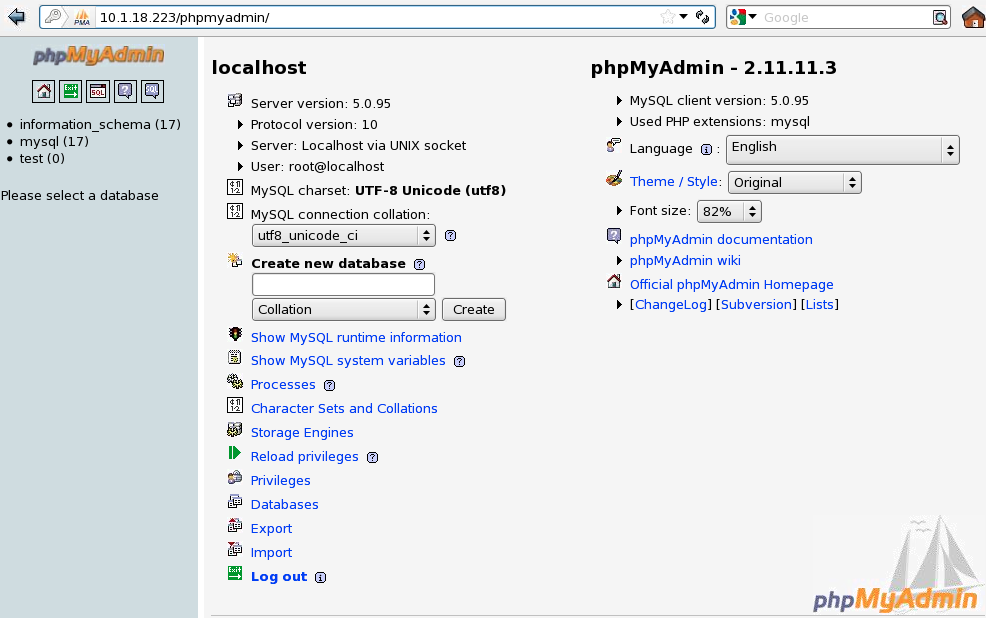
\includegraphics[width=1.0\textwidth]{images/phpmyadmin.png}
				\caption{phpMyAdmin front page}
			\end{centering}
		\end{figure}

\end{itemize}

\lineparagraph{Database Implementation}
The final step of the database development is the physical implementation. The tool phpMyAdmin is used to implement the database at the MySQL server the code blocks generated by this tools are described bellow. 
\\
The following blocks of code create the database and tables in it.
% Create database directory
\lineparagraph{Database}
To create tables that can be used to store data, a database directory have to be created.
		\begin{lstlisting}[language=sql, stepnumber=0, tabsize=1]
			CREATE DATABASE `powersystem`;
		\end{lstlisting}
		With the database directory created, the tables can now be created inside this directory.
% Create tables
\lineparagraph{Tables}
The SQL syntax is going to be explain for only one table since the other tables will follow the same syntax just using different names.\\
		MODULES
		\begin{lstlisting}[language=sql, stepnumber=0, tabsize=1]
			CREATE TABLE `powersystem`.`MODULES` (
				`ID_MODULE` INT NOT NULL AUTO_INCREMENT ,
				`UNIQUE_ID` INT NOT NULL ,
				`ID_TYPE` TINYINT NOT NULL ,
				`ID_STATUS` TINYINT NOT NULL ,
				`NAME` VARCHAR( 50 ) NOT NULL ,
				PRIMARY KEY ( `ID_MODULE` , `UNIQUE_ID` )
			) 
		\end{lstlisting}
		This block of code will create the table MODULES in the database directory 'powersystem' with the columns ID\_MODULE and UNIQUE\_ID as primary key for this table. Primary keys are columns where one and only one value is allowed, in this table UNIQUE\_ID is important to exist only once. 
		ID\_TYPE and ID\_STATUS are foreigner keys form table TYPES and STATUS and NAME is the name of the module as explained in the analysis phase.
		TYPES
		\begin{lstlisting}[language=sql, stepnumber=0, tabsize=1]
			CREATE TABLE `powersystem`.`TYPES` (
			`ID_TYPE` INT NOT NULL AUTO_INCREMENT PRIMARY KEY ,
			`TYPES` VARCHAR( 50 ) NOT NULL
			)
		\end{lstlisting}
		STATUS
		\begin{lstlisting}[language=sql, stepnumber=0, tabsize=1]
			CREATE TABLE `powersystem`.`STATUS` (
			`ID_STATUS` INT NOT NULL  AUTO_INCREMENT,
			`STATUS` VARCHAR( 50 ) NOT NULL ,
			PRIMARY KEY ( `ID_STATUS` )
			)
		\end{lstlisting}	
		SENSORS
		\begin{lstlisting}[language=sql, stepnumber=0, tabsize=1]
			CREATE TABLE `powersystem`.`SENSORS` (
			`ID_MODULE` INT NOT NULL AUTO_INCREMENT ,
			`ID_SENSOR` INT NOT NULL ,
			`ID_UNITS` INT NOT NULL ,
			PRIMARY KEY ( `ID_MODULE` , `ID_SENSOR` )
			)
		\end{lstlisting}
		UNITS
		\begin{lstlisting}[language=sql, stepnumber=0, tabsize=1]
			CREATE TABLE `powersystem`.`UNITS` (
			`ID_UNIT` INT NOT NULL ,
			`UNIT` VARCHAR( 50 ) NOT NULL ,
			PRIMARY KEY ( `ID_UNIT` )
			)
		\end{lstlisting}
		WRAPPER
		\begin{lstlisting}[language=sql, stepnumber=0, tabsize=1]
			CREATE TABLE `powersystem`.`WRAPPER` (
			`ID_WRAP` INT NOT NULL AUTO_INCREMENT PRIMARY KEY ,
			`DATE_FROM` DATETIME NOT NULL ,
			`DATE_TO` DATETIME NOT NULL ,
			`ID_SENSOR` INT NOT NULL ,
			`VALUE` FLOAT NOT NULL
			)
		\end{lstlisting}
		LOGS
		\begin{lstlisting}[language=sql, stepnumber=0, tabsize=1]
			CREATE TABLE `powersystem`.`LOGS` (
			`ID_LOG` INT NOT NULL AUTO_INCREMENT PRIMARY KEY ,
			`ID_SENSOR` INT NOT NULL ,
			`DATE_TIME` DATETIME NOT NULL ,
			`HUB_PORT` INT NOT NULL ,
			`VALUE` FLOAT NOT NULL
			)
		\end{lstlisting}
	
% Populate Tables
\lineparagraph{Populate Tables}
The tables are populated using phpMyAdmin since the easy implementation with this tool. All the SQL syntax generated by this tools is shown and explained bellow.
Tables are populated in the beginning with initial values known values. PHP scripts will allow later on to add new data to this tables, allowing the system to be more flexible to unknown data.\\
		STATUS:
		This SQL code block insert tree value into the table status in the powersystem database directory.
		\begin{lstlisting}[language=sql, stepnumber=0, tabsize=1]
			INSERT INTO `powersystem`.`STATUS` (`ID_STATUS` ,`STATUS`	)
			VALUES (NULL , 'Running'),
			(NULL , 'Stoped'),
			(NULL , 'Warning');
		\end{lstlisting}
		TYPES
		\begin{lstlisting}[language=sql, stepnumber=0, tabsize=1]
			INSERT INTO `powersystem`.`TYPES` (`ID_TYPE` ,`TYPES`)
			VALUES (NULL , 'Input'), 
			(NULL , 'Output'),
			(NULL , 'Bidirectional');
		\end{lstlisting}
		UNITS
		\begin{lstlisting}[language=sql, stepnumber=0, tabsize=1]
			INSERT INTO `powersystem`.`UNITS` (`ID_UNIT` ,`UNIT`)
			VALUES (NULL , 'V'),
			(NULL , 'A'),
			(NULL , 'deg'), 
			(NULL , 'm/s'), 
			(NULL , 'km/h'), 
			(NULL , 'N'), 
			(NULL , 'P');
		\end{lstlisting}		

%	        Verification
%	
%	                Module tests
%	                Integration tests
%	                Acceptance test
\subsubsection{Verification}
\begin{table}[H]
\centering
	\begin{tabular}{| c | l | c |}
		\hline
		Verification & Description & Acceptance \\\hline
		1 & Initialise a new module or identify if the module was connected before & ~ \\\hline
		2 & Change the status for each module & ~ \\\hline
		3 & Add new measurements for each module & ~ \\\hline
		4 & Decrease the database size using a time span and average values. & ~ \\\hline
		5 & Web server running and accessible & Ok \\\hline
		6 & MySQL server running and accessible) & Ok \\\hline
		7 & PHP script language testing & Ok \\\hline
		8 & phpMyAdmin tool installed and running & Ok \\\hline
		9 & Database created & Ok \\\hline
		10 & Tables created & Ok \\\hline
		11 & Tables populated & Ok \\\hline
		2 & Change the status for each module & ~ \\\hline
		2 & Change the status for each module & ~ \\\hline
		2 & Change the status for each module & ~ \\\hline
		2 & Change the status for each module & ~ \\\hline
		2 & Change the status for each module & ~ \\\hline
		2 & Change the status for each module & ~ \\\hline
		2 & Change the status for each module & ~ \\\hline
		2 & Change the status for each module & ~ \\\hline
		2 & Change the status for each module & ~ \\\hline
	\end{tabular}
\end{table}
%%%%%%%%%%%%%%%%%%%%%%%%%%%%%%%%
\subsubsection{Database Structure}
This documentation is generated by phpMyAdmin running on linux CENTOS server.
\begin{lstlisting}[language=sql, stepnumber=0, tabsize=1]
-- phpMyAdmin SQL
-- version 2.11.11.3
-- http://www.phpmyadmin.net
--
-- Host: localhost
-- Generation Time: Mar 29, 2012 at 04:11 PM
-- Server version: 5.0.95
-- PHP Version: 5.1.6
--
-- Database: `powersystem`
--
-- --------------------------------------------------------
--
-- Table structure for table `LOGS`
--
CREATE TABLE `LOGS` (
  `ID_LOG` int(11) NOT NULL auto_increment,
  `ID_SENSOR` int(11) NOT NULL,
  `DATE_TIME` datetime NOT NULL,
  `HUB_PORT` int(11) NOT NULL,
  `VALUE` float NOT NULL,
  PRIMARY KEY  (`ID_LOG`)
) ENGINE=MyISAM DEFAULT CHARSET=latin1 AUTO_INCREMENT=1 ;
--
-- --------------------------------------------------------
--
-- Table structure for table `MODULES`
--
CREATE TABLE `MODULES` (
  `ID_MODULE` int(11) NOT NULL auto_increment,
  `UNIQUE_ID` int(11) NOT NULL,
  `ID_TYPE` tinyint(4) NOT NULL,
  `ID_STATUS` tinyint(4) NOT NULL,
  `NAME` varchar(50) NOT NULL,
  PRIMARY KEY  (`ID_MODULE`,`UNIQUE_ID`)
) ENGINE=MyISAM DEFAULT CHARSET=latin1 AUTO_INCREMENT=1 ;
--
-- --------------------------------------------------------
--
-- Table structure for table `SENSORS`
--
CREATE TABLE `SENSORS` (
  `ID_MODULE` int(11) NOT NULL auto_increment,
  `ID_SENSOR` int(11) NOT NULL,
  `ID_UNITS` int(11) NOT NULL,
  PRIMARY KEY  (`ID_MODULE`,`ID_SENSOR`),
  KEY `ID_MODULE` (`ID_MODULE`)
) ENGINE=MyISAM DEFAULT CHARSET=latin1 AUTO_INCREMENT=1 ;
--
-- --------------------------------------------------------
--
-- Table structure for table `STATUS`
--
CREATE TABLE `STATUS` (
  `ID_STATUS` int(11) NOT NULL auto_increment,
  `STATUS` varchar(50) NOT NULL,
  PRIMARY KEY  (`ID_STATUS`)
) ENGINE=MyISAM  DEFAULT CHARSET=latin1 AUTO_INCREMENT=4 ;
--
--
INSERT INTO `STATUS` (`ID_STATUS`, `STATUS`) VALUES
(1, 'Running'),
(2, 'Stoped'),
(3, 'Warning');
--
-- --------------------------------------------------------
--
-- Table structure for table `TYPES`
--
CREATE TABLE `TYPES` (
  `ID_TYPE` int(11) NOT NULL auto_increment,
  `TYPES` varchar(50) NOT NULL,
  PRIMARY KEY  (`ID_TYPE`)
) ENGINE=MyISAM  DEFAULT CHARSET=latin1 AUTO_INCREMENT=4 ;
--
--
INSERT INTO `TYPES` (`ID_TYPE`, `TYPES`) VALUES
(1, 'Input'),
(2, 'Output'),
(3, 'Bidirectional');
--
-- --------------------------------------------------------
--
-- Table structure for table `UNITS`
--
CREATE TABLE `UNITS` (
  `ID_UNIT` int(11) NOT NULL auto_increment,
  `UNIT` varchar(50) NOT NULL,
  PRIMARY KEY  (`ID_UNIT`)
) ENGINE=MyISAM  DEFAULT CHARSET=latin1 AUTO_INCREMENT=8 ;
--
--
INSERT INTO `UNITS` (`ID_UNIT`, `UNIT`) VALUES
(1, 'V'),
(2, 'A'),
(3, 'deg'),
(4, 'm/s'),
(5, 'km/h'),
(6, 'N'),
(7, 'P');
-- --------------------------------------------------------
--
-- Table structure for table `WRAPPER`
--

CREATE TABLE `WRAPPER` (
  `ID_WRAP` int(11) NOT NULL auto_increment,
  `DATE_FROM` datetime NOT NULL,
  `DATE_TO` datetime NOT NULL,
  `ID_SENSOR` int(11) NOT NULL,
  `VALUE` float NOT NULL,
  PRIMARY KEY  (`ID_WRAP`)
) ENGINE=MyISAM DEFAULT CHARSET=latin1 AUTO_INCREMENT=1 ;
--
--
		\end{lstlisting}	
%%%%%%%%%%%%%%%%%%%%%%%%%%%%%%%%


\subsection{Physical interface - Theis}
The interface shall be made to fulfil the requirements \textit{NF-1.5}\footnote{Requirement is found in table 3.2 in EPRO 3 project energy-hub} and \textit{B-1.2}\footnote{Requirement is found in table 3.4 in EPRO 3 project energy-hub}.\\
\begin{table}[H]
\centering
	\begin{tabular}{|p{1.2cm}|p{2.3cm}|p{6cm}|p{6cm}|}
	\hline
	ID		& Requirement	& Description															& Comments\\\hline
	NF-1.5	& HW Interface	& 1 start button for the hub. 10 buttons to each start a module.		& This is shown with 8 switches on the Spartan 6 board\\\hline
	B-1.2	& Physical		& 1 diode showing when a module is off and one showing when it is on.	& This is shown with 8 LEDs on the Spartan 6 board\\\hline
	\end{tabular}
\end{table}

\subsubsection{Analysis}
The physical interface is where the user interact directly with the hub, it is placed on the hub cabinet. It shall be possible for the user to start the hub and modules. There shall also be an indication of the hub and module status.\\
For turning on module there shall be a switch for each module and one for turning on the hub. To indicate the status there shall be a LED for every module and one to indicate the hub status.\\
The interface is made on the Spartan6 and is communicating with the ARM7 through the external memory controller in the ARM7 and using a wishbone interface on the Spartan6.
\begin{figure}[H]
	\begin{centering}
		%\missingfigure{Updated timebox figure}
		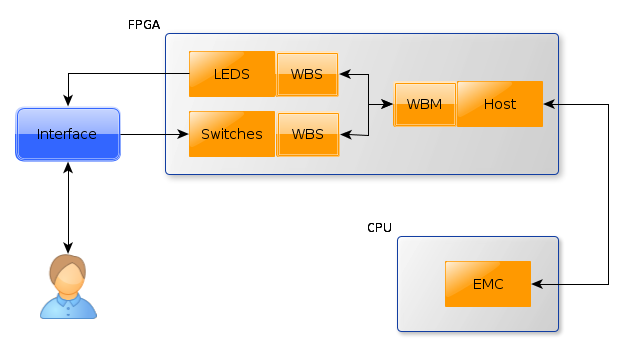
\includegraphics[width=1.0\textwidth]{images/analysis_phy_interface.png}
		\caption{User-system interface interaction}
	\end{centering}
\end{figure}
\subsubsection{Design}
The physical interface is made with 8 switches and 8 LEDs, and is controlled through the Spartan 6. The block diagram below shows how the interface is made inside the Spartan 6, with the wishbone interface to the master, the master wishbone is discussed in Time box 3 section 3.5.3.
\begin{figure}[H]
	\begin{centering}
			%\missingfigure{Updated timebox figure}
			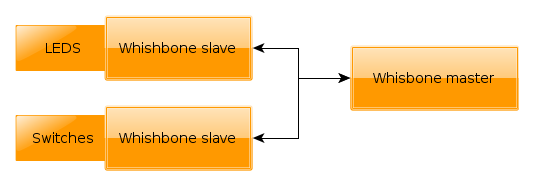
\includegraphics[width=0.7\textwidth]{images/Design_HWmodule.png}
			\caption{Block diagram for the interface in the Spartan 6}
	\end{centering}
\end{figure}
\subsubsection{Implementation}
The implementation is made in the Spartan 6 board. There is 8 LEDs and 8 switches on board, that is used for the interface. The blocks is written in VHDL.
\paragraph{LED interface}
The LEDs is controlled with the LED block in the Spartan 6, and it is able to send and receive data with a wishbone interface. The data output is the status of the 8 LEDs, the data input is used to turn on and off the LEDs.\\\\
In the code below, the entity of the LED controller is shown, the wishbone interface is defined from line 5 to line 16, these lines is common for all wishbone slaves. In line 19 the output for the 8 LEDs is defined as a 8 bit vector.
\begin{lstlisting}[language=VHDL]
...
entity WBS_leds is
	port	(
			--! Wishbone Slave interface
			--Input
			clk_i			: in		std_logic;		--! Clock input from SYSCON
			rst_i			: in		std_logic;		--! Reset for Wishbone interface
			cyc_i			: in		std_logic;		--! cycle input, asserted when cycle is in progress
			stb_i			: in		std_logic;		--! Strobe input, similar to Chip Select
			we_i			: in		std_logic;		--! Write Enable: High=WR, Low=RD
			dat_i			: in		wb_dat_typ;		--! data from host
			adr_i			: in		wb_lad_typ;		--! Low address input
			--Ouput
			ack_o			: out		std_logic;		--! Slave acknowledge output, asserted after sucessful cycle
			err_o			: out		std_logic;		--! Error output, abnormal cycle termination
			rty_o			: out		std_logic;		--! Retry output, slave not ready
			dat_o			: out		wb_dat_typ;		--! data to host
			---------------------------------
			--! Output port
			leds			: out		std_logic_vector(7 downto 0)
			);
end WBS_leds;
...
\end{lstlisting}
Here the slave is responding the master, the error and retry signal is not supported in this slave, they are assigned with zeros, the acknowledge bit is set high if the strobe and cycle is assigned by the master. The Q signal is assigned to the LEDs and the data output. If the master reads data, it will get the status of the LEDs.
\begin{lstlisting}[language=VHDL]
...
	signal Q				: std_logic_vector(7 downto 0);

begin

--  Concurrent assignments
--	Wishbone cycle acknowledge
	err_o <= '0';	--error signal
	rty_o <= '0';	--retry signal
	ack_o <= stb_i and cyc_i;  --! asynchronous cycle termination is OK here.
--	Data
	dat_o(7 downto 0) <= Q;
	leds <= Q;
...
\end{lstlisting}
In the code below the writing to the LEDs is made. If the cycle, strobe and the write enable inputs is high, the master wants to write data to this slave, then the process checks the address that the slave is sending data to. To write data to the LEDs the address has to be five zeros, then the code will assign Q with the data input from the master.
\begin{lstlisting}[language=VHDL]
...
--!  Processes                                             --
--! Wishbone write to Q register
	Reg : process(clk_i)
		begin
			if(clk_i'event and clk_i = '1') then
				if (rst_i = '1') then
					Q <= Revision_c(7 downto 0);          --! Revision readable at reset 
				else
					if ((cyc_i and stb_i and we_i) = '1') then
						case adr_i is
							when A_WBO_REG1 =>
								Q	<= dat_i(7 downto 0);
							when others =>
							--Ack_o <= '0'; 
						end case;
						
					else
						Q <= Q;
					end if;
				end if;
			end if;
	end process Reg;
...
\end{lstlisting}
\paragraph{Switch interface}
The switches is read from the switches block through wishbone interface in the Spartan 6. This block is read only, and the data output is the status of the 8 switches.\\\\
The wishbone part of the code i common to the entity code in the LED block. For the switches an input vector is made with 8 bit.
\begin{lstlisting}[language=VHDL]
...
entity WBS_switches is
	port	(
			--! Wishbone Slave interface
			--Input
			clk_i			: in		std_logic;		--! Clock input from SYSCON
			rst_i			: in		std_logic;		--! Reset for Wishbone interface
			cyc_i			: in		std_logic;		--! cycle input, asserted when cycle is in progress
			stb_i			: in		std_logic;		--! Strobe input, similar to Chip Select
			we_i			: in		std_logic;		--! Write Enable: High=WR, Low=RD
			dat_i			: in		wb_dat_typ;		--! data from host
			adr_i			: in		wb_lad_typ;		--! Low address input
			--Ouput
			ack_o			: out		std_logic;		--! Slave acknowledge output, asserted after sucessful cycle
			err_o			: out		std_logic;		--! Error output, abnormal cycle termination
			rty_o			: out		std_logic;		--! Retry output, slave not ready
			dat_o			: out		wb_dat_typ;		--! data to host
			-------------------------------------------------
			--! Intput port
			sw				:in			std_logic_vector(7 downto 0)
			);
end WBS_switches;
...
\end{lstlisting}
The acknowledge bit for the master is set here with the high strobe and cycle input.
\begin{lstlisting}[language=VHDL]
...
--  Concurrent assignments
--	Wishbone cycle acknowledge
	err_o <= '0';	--error signal
	rty_o <= '0';	--retry signal
	ack_o <= stb_i and cyc_i;  --! asynhronous cycle termination is OK here.
...
\end{lstlisting}
In the code below, the switches status is written to the master wishbone. The process write the switches status to the lowest 8 bit in the data string and fill the rest with zeros, if the cycle and strobe input are high and the write enable is low to indicate that the master wants to read data.
\begin{lstlisting}[language=VHDL]
...
--!  Processes                                             --
	Reg : process(clk_i)
		begin
			if(clk_i'event and clk_i = '1') then
				if (rst_i = '1') then
					dat_o <= Revision_c;          --! Revision readable at reset
				else
					if ((cyc_i and stb_i and not we_i) = '1') then
						case adr_i is
							when A_WBO_REG1 =>
								dat_o(7 downto 0)	<= sw;
								dat_o(15 downto 8)	<= (others => '0');
							when others =>
							--Ack_o <= '0'; 
						end case;
						
					else
						dat_o <= dat_o;
					end if;
				end if;
			end if;
	end process Reg;
...
\end{lstlisting}
The rest of the code is made by Morten Opprud Jakobsen, and is not in the scope of this section.
\subsubsection{Verification}
The verification is made on the computer by simulating a test bench for writing to the LEDs and reading from the switches, and a test program on the ARM7 is made, to read the switches and write the status to the LEDs. The test with the ARM7 was recorded and is available through this link \url{http://www.youtube.com/watch?v=3MUK6qbg0Rk}
\paragraph{Read switches}
In the start of the test, \textit{reset} is active and the switch status is set. before a read cycle is assigned the \textit{address} is assigned, then the \textit{chip select} goes low, then \textit{read (output enable)}. The test shows that the data is tri-stated until the \textit{read} goes low, and one clock cycle after, the status on \textit{switch} is loaded into \textit{data}.
\begin{figure}[H]
	\begin{centering}
		%\missingfigure{Updated timebox figure}
		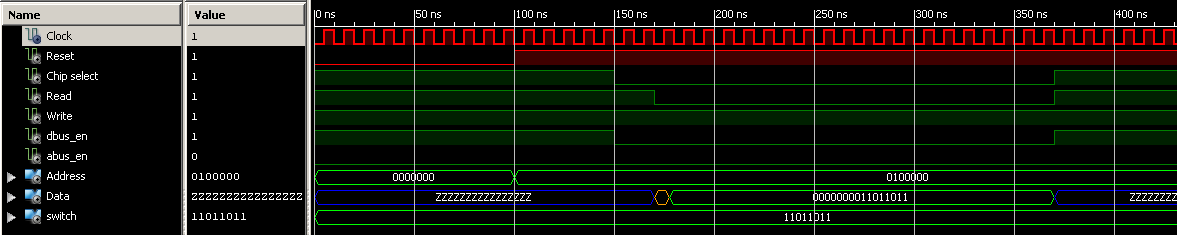
\includegraphics[width=1.0\textwidth]{images/tb_wb_read.png}
		\caption{Test bench simulation of read}
	\end{centering}
\end{figure}
\paragraph{Write to LEDs}
In the write test, \textit{leds} is uninitialized and \textit{reset} is active, before a write cycle is assigned the \textit{address} and \textit{data} is assigned, then the \textit{chip select} goes low, then \textit{write (write enable)}. The test show that one clock cycle after \textit{write} goes low the \textit{data} is loaded onto the \textit{Leds}.
\begin{figure}[H]
	\begin{centering}
		%\missingfigure{Updated timebox figure}
		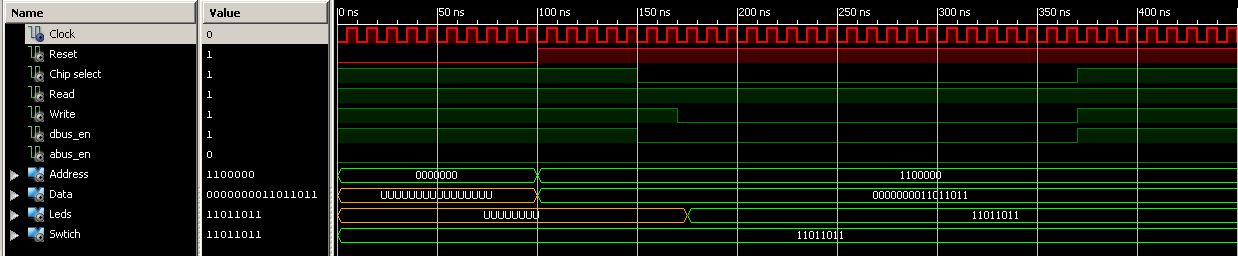
\includegraphics[width=1.0\textwidth]{images/tb_wb_write.png}
		\caption{Test bench simulation of write}
	\end{centering}
\end{figure}
\subsubsection{Conclusion}
The test verify that the implementation of the interface design is working properly. The switches block is not completely finished, right now to register changes in the switches the ARM7 shall read the status to often, to prevent this an interrupt function is to be implemented, in that way the ARM7 is only reading the status when the switches changes. The interrupt function is not on the scope of this time box.
\subsection{Deployment}
%			Customers signature for acceptance 
